\chapter{Motor Learning in Virtual Reality}
\label{chapter:theoretical_background}
This chapter provides the theoretical background of Mixed Reality, Motor Learning, Visual Perspectives and handling physical load. These are the most important aspects that serve as the foundation for the proposed study design. Finally, an analysis of related work is provided. This chapter gives insights into how this work is informed and differentiated by other researchers.

\section{Mixed Reality}
\label{section:mixed_reality}
Milgram and Kishinho~\cite{mrcontinuum} describe Mixed Reality for visual displays on a continuum (see seminar thesis chapter 2.3). Virtual Reality is purely digital, and thereby the environment is blocked entirely. In Augmented Reality, the environment is visible and augmented with digital elements. During Motor Learning, the visual perception of the own body is desirable. Though, the approach of augmenting the real-world body with a virtual guidance visualisation is promising. However, today's AR-technology provides a small field of view. A solution to this could be the video see-through technology, but it is limited by latency and distortion.\\
The body's perception can also be achieved by tracking the learner's body and render it over the learner's physical body. Though, the visual perception of the learner's body can be established in VR. Consequentially, this work will focus on Motor Learning in Virtual Reality.

\section{Motor Learning}
\label{section:motor_learning}
Motor Learning is achieved through instruction, trying, imitation or a combination of them~\cite{mlbook}. The process of Motor Learning can be divided into three parts: cognitive stage, associative stage and autonomous stage. In the cognitive stage, training methods are most efficient, and the performance gain ist the highest among the stages~\cite{mlbook}. Tasks that belong to this stage are thereby best suited for a study. A detailed description of the stages can be found in the preceding seminar thesis chapter 2.2.\\
Movements can be classified by two means: by the \textit{particular movements} and based on the \textit{perceptual attributes}. Based on the \textit{particular movements}, the classification is described by a continuum, compare figure~\ref{fig:movement_classification} left. On the extremes of the continuum are discrete movements and continuous movements. Between these extremes, serial movements are located. Discrete movements are too short for an evaluation. Continuous movements do not have a recognisable beginning, and thereby they are not suitable for the study in question either. Serial movements are chained discrete movements with a recognisable beginning and end. This allows a task decomposition and an evaluation of particular sub-tasks. Discrete movements are widely used for research in Motor Learning, for example~\cite{lightguide,mythaichicoaches,elearningma}; therefore, the study task design is based on discrete movements.\\
The classification based on the \textit{perceptual attributes} is also represented by a continuum and includes the environment in which the movement is performed, compare figure~\ref{fig:movement_classification} right. At the extremes of the continuum, open skills and closed skills are located. For closed skills, the environment is predictable, while in open skills, the environment is not predictable. The study aims to analyse the learners' performance of following a movement and not how they can adapt to environmental changes. Thereby, this study's task must be located on the left-hand side of the continuum: closed skills.
\begin{figure}[htb]
	\centering
	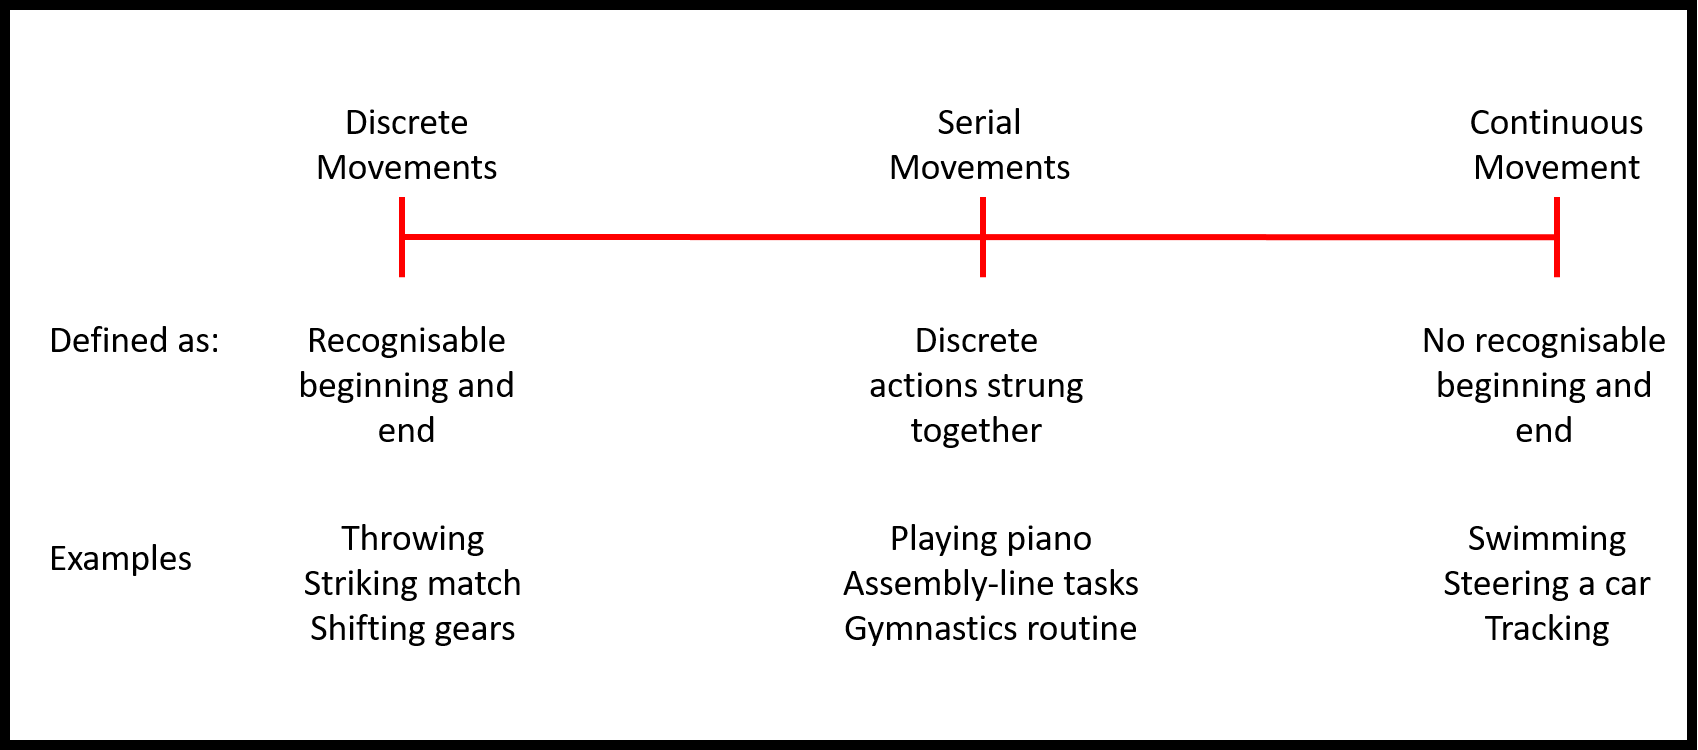
\includegraphics[width=0.49\textwidth]{figures/movement_classification.png}
	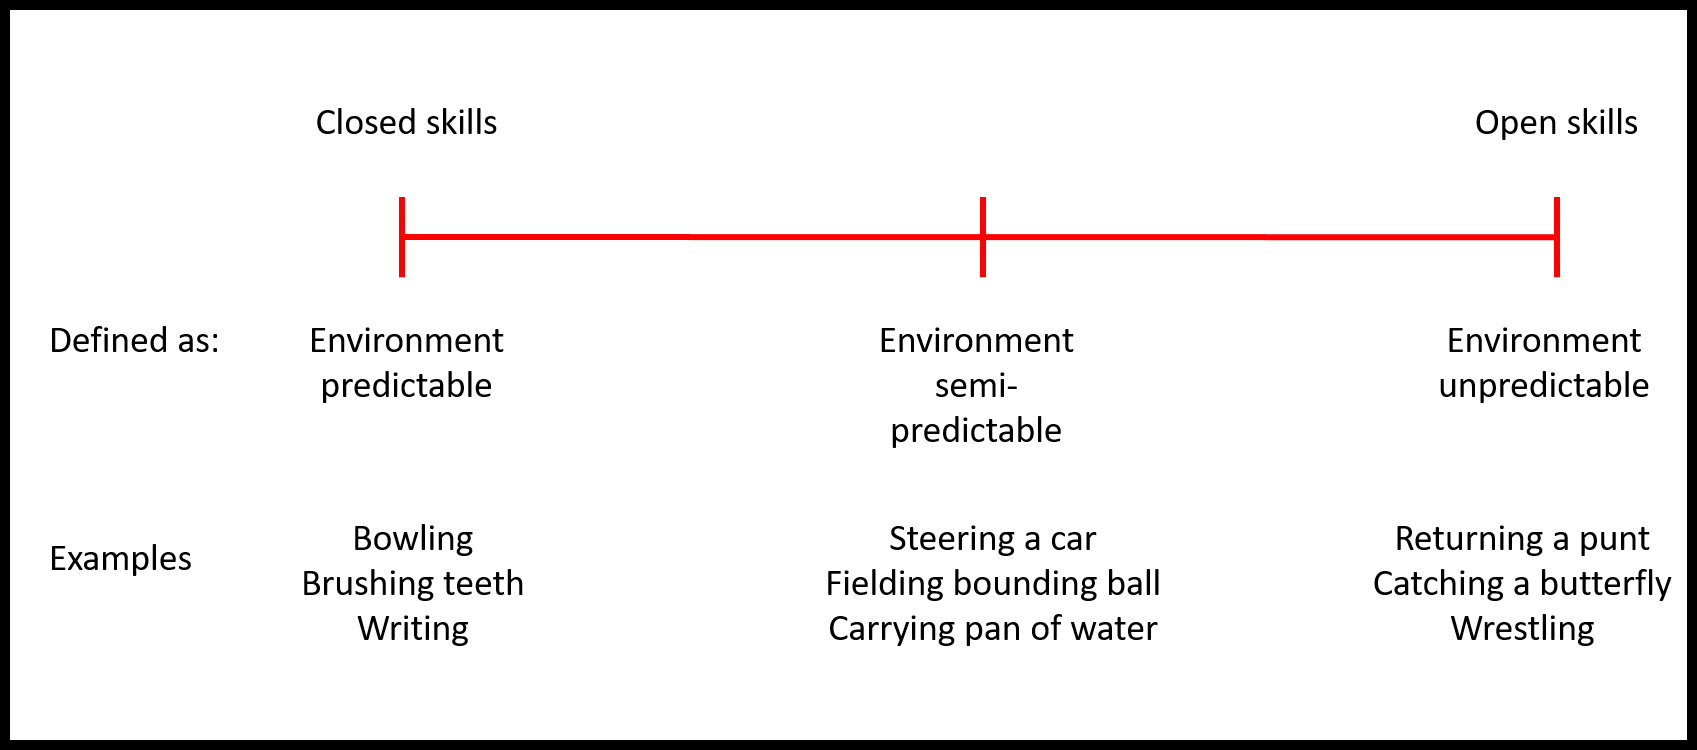
\includegraphics[width=0.49\textwidth]{figures/movement_classification2.png}
	\caption[Movement classifications by Scmidt et al.]{Movement classification by \textit{particualar movements} (left) and \textit{perceptual attributes} by Smift at al.~\cite{mlbook}}
	\label{fig:movement_classification}
\end{figure}

\subsection{Measurements for Motor Learning}
\label{section:measures_for_ml}
The movements of a teacher and the movement of a learner differ. To assess the difference between the two movements, two main classes of measures can be applied~\cite{mlbook}: \textit{measures of error for a single object} and \textit{measures of time and speed}.
\textit{Measure of error for a single object} represent the degree to which the target movement is amiss. Schmidt et al.~\cite{mlbook} provide five \textit{error measures} to calculate this error, compare seminar thesis chapter 2.2. \textit{Constant Error} is the most common measure in related work to determine the difference between the movement of the learner and the movement of the teacher, for example~\cite{perspectivematters,thaichichua,YouMove,onebody,vrdancetrainer,lightguide,physioathome}. Constant Error is defined as the average error between the movement of the learner and the movement of the teacher and is described as
\begin{equation}
	\label{eq:constanterror}
	CE=\frac{\sum_i(x_i-T)}{n}
\end{equation}
with $x_i$: actual value, $T$: target value, $n$: number of values~\cite{mlbook}.\\
The basic idea of \textit{measures of time and speed} is that a performer who can accomplish more in a given amount of time or who can accomplish a given amount of behaviours in less time is more skilful. In related work, this measure is mostly assessed by the task completion time, for example~\cite{perspectivematters,onebody,lightguide}.


\section{Visual Perspectives}
\label{section:visual_perspectives}
Wang and Milgram~\cite{centricitycontinuum} describe visual perspectives by the \textit{centricity continuum}~\ref{fig:ego-exo-continuum}. On the left extreme on the continuum, the ego-centric visual perspective is located; on the right extreme, the exo-centric visual perspective can be found, while the middle part represents tethered visual perspectives. By moving from the left to the right, the so-called \textit{tethering distance} increases. The \textit{tethering distance} describe the distance of the anchor point of the eyes to the object to control. In this work, the object to control is the human-shaped guidance visualisation (avatar). Furthermore, Wang and Milgram distinguish tethered visual perspective in dynamic and rigid. A detailed description is given in the seminar thesis chapter 2.1. 
\begin{figure}[htb]
	\centering
	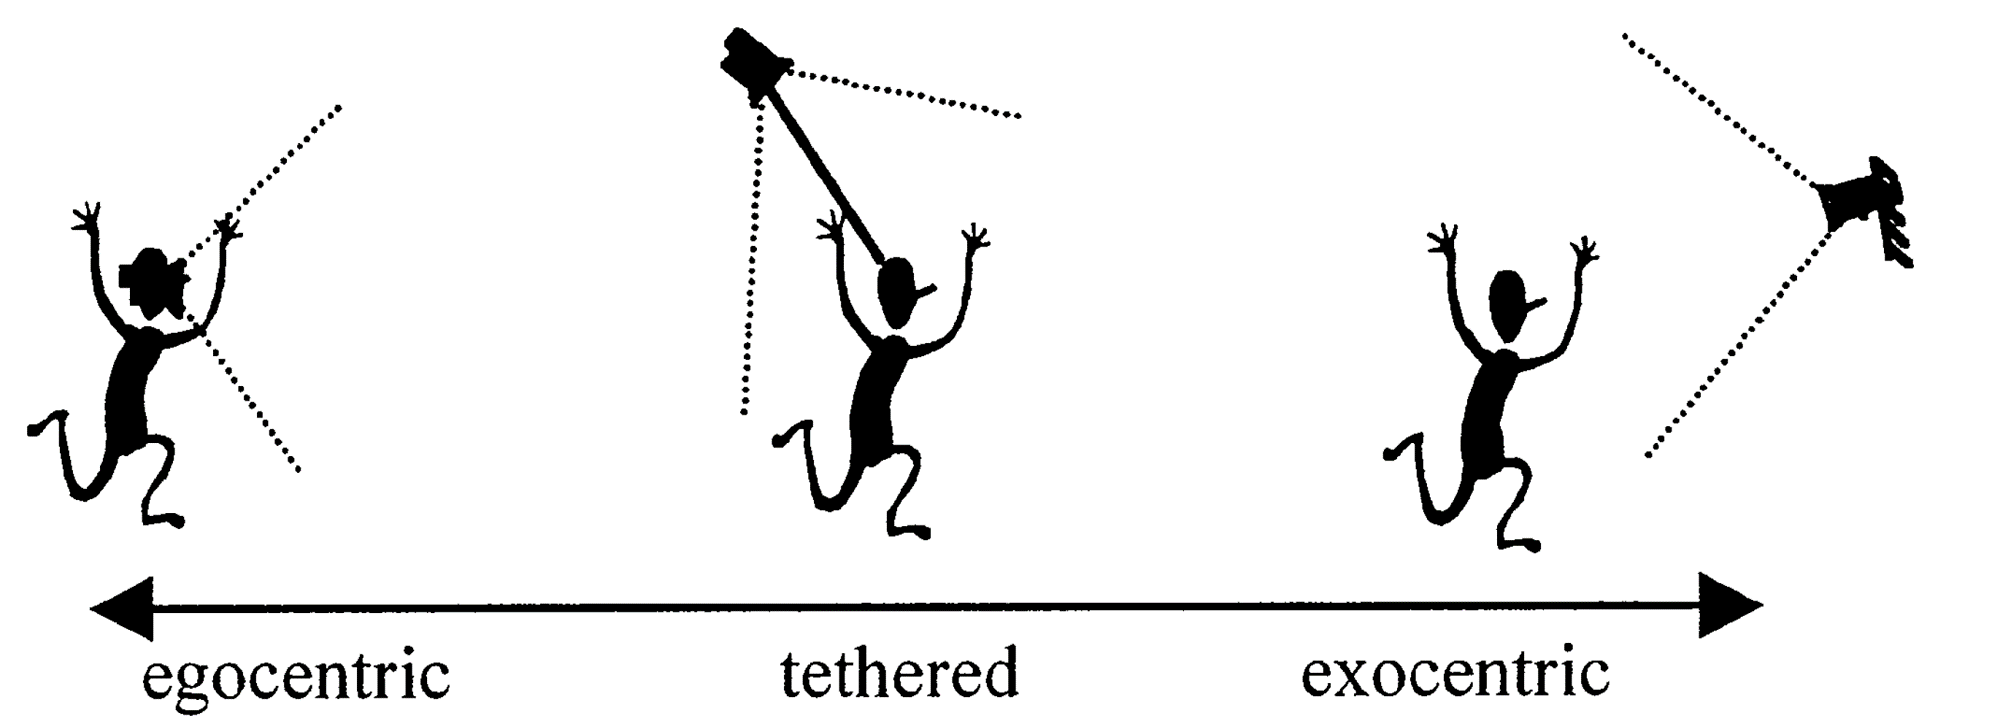
\includegraphics[width=\textwidth]{figures/ego_exo_continuum.PNG}
	\caption[Centricity continuum]{Centricity continuum by Wang and Milgram~\cite{centricitycontinuum}}
	\label{fig:ego-exo-continuum}
\end{figure}
Given a scenario where one learner mimics the movement of one teacher, five different visual perspectives are possible:
\begin{figure}[htb]
	\centering
	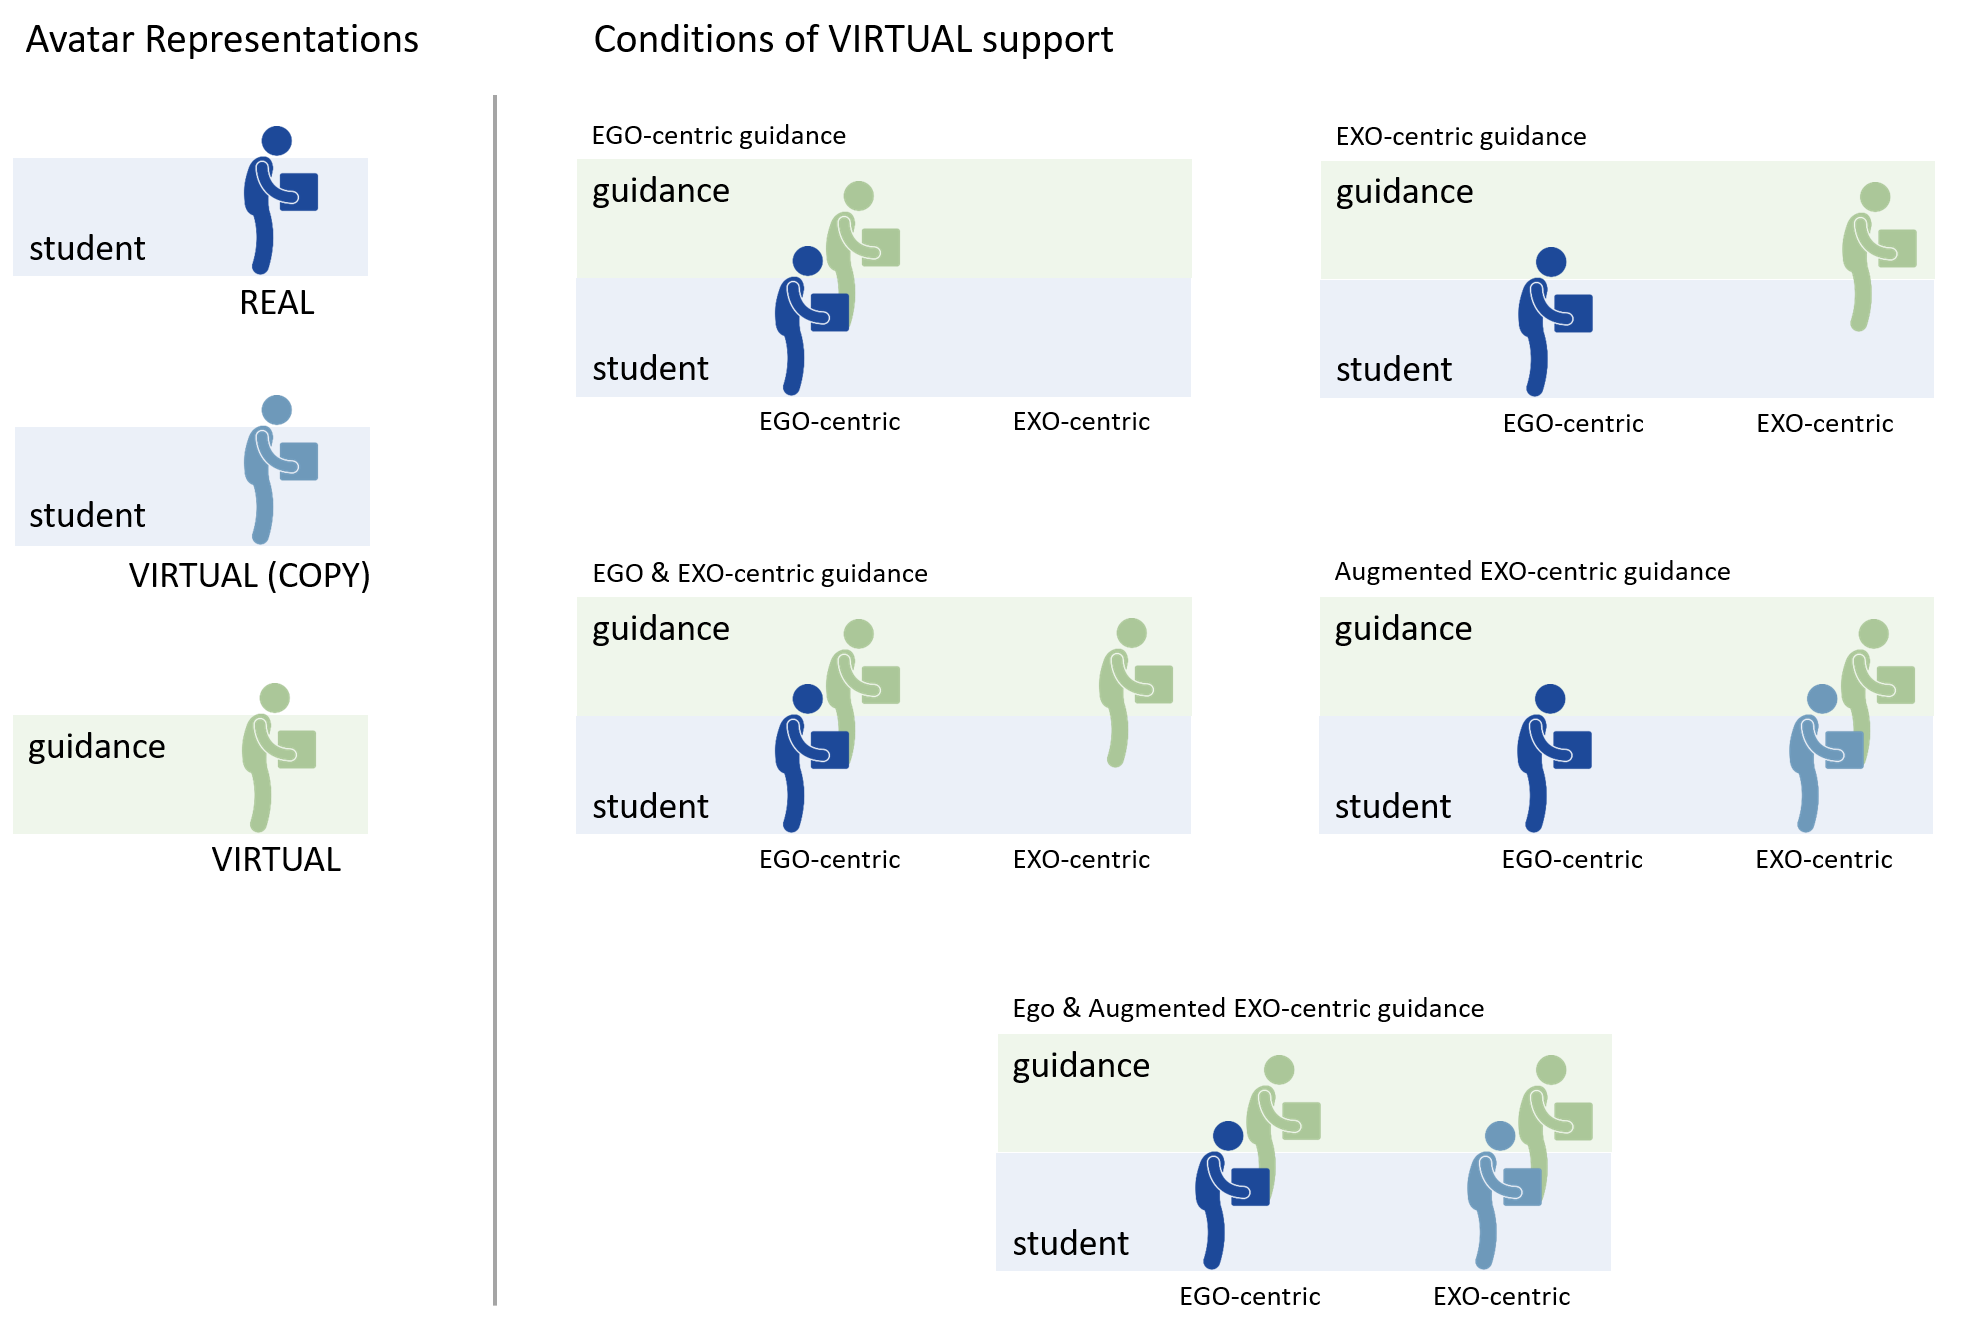
\includegraphics[width=\textwidth]{figures/perspectives.png}
	\caption[Possible perspectives]{Possible perspectives with one real-world student and one real-world teacher.}
	\label{fig:perspectives}
\end{figure}
\begin{itemize}
	\item \textbf{Ego-centric}: the avatar of the teacher is located inside the body of the avatar of the learner; the learner sees the guidance visualisation inside the own body, compare figure~\ref{fig:perspectives} top left.
	\item \textbf{Exo-centric}: the avatar of the guidance visualisation is located outside of the avatar of the learner; the learner sees the guidance visualisation, e.g. in front of him/her, compare figure~\ref{fig:perspectives} top right.
	\item \textbf{Ego \& exo-centric}: the combination of ego-centric and exo-centric. The learner sees the guidance visualisation as well as inside and outside of the own body, compare figure~\ref{fig:perspectives} middle left.
	\item \textbf{Augmented exo-centric}: the guidance visualisation is located outside of the learner's avatar. Additionally, a virtual copy of the student is located inside the exo-centric guidance visualisation, compare figure~\ref{fig:perspectives} middle right.
	\item \textbf{Ego \& augmented exo-centric}: the combination of the ego-centric visual perspective and the augmented exo-centric visual perspective; the learner sees the guidance visualisation inside the own body, as well as outside. Additionally, a virtual copy of the learner is located inside the exo-centric guidance visualisation, compare figure~\ref{fig:perspectives} bottom.	
\end{itemize}

\section{Handling Physical Load - chang to mmh}
\label{section:handlingphysicalload}
The handling of physical load is composed of five elemental tasks: lift, lower, push, pull and hold~\cite{mmh}. Additionally, there are non-elemental tasks like turning and sliding, ibid.. This work will use a study tasks that include the handling of physical load. Evidently, the task should consist of these elemental tasks. A task that consists of elemental tasks can be generalised to other tasks to a certain extend. To gain a stronger data basis by repeating, multiple elemental tasks can be chained together, to form a so-called Unit-Combined-MMH, ibid.. In chapter~\ref{sec:task_design} is described how the elemantal tasks become sub-tasks of the study task.

\section{Ergonomic Risk Measurements}
\label{section:rm}
Risk Measurements (RM)

\section{Related Work: Motor Learning in Virtual Reality}
\label{section:related_work}
Training movements in Virtual Reality was investigated previously in several works. The preceding seminar thesis (see chapter 3) provided an overview over 23 (compare table~\ref{tab:rw_overview}) of these works and evaluated six of them in detail: Tai Chi Trainer by Chua et al.~\cite{thaichichua}, YouMove by Anderson et al.~\cite{YouMove}, VR Dance Trainer by Chan et al.~\cite{vrdancetrainer}, OneBody by Hoang et al.~\cite{onebody}, LightGuide by Sodhi et al.~\cite{lightguide} and Pyhsio@Home by Tang et al.~\cite{physioathome}. Special attention was paid to the visual perspective, task, guidance visualisation and their independent and dependent variables they used in their investigations. Finally, the results of these works were concluded. An overview is depicted in table~\ref{tab:rw_overview_detail}.
\begin{table}[htb]
	\centering
	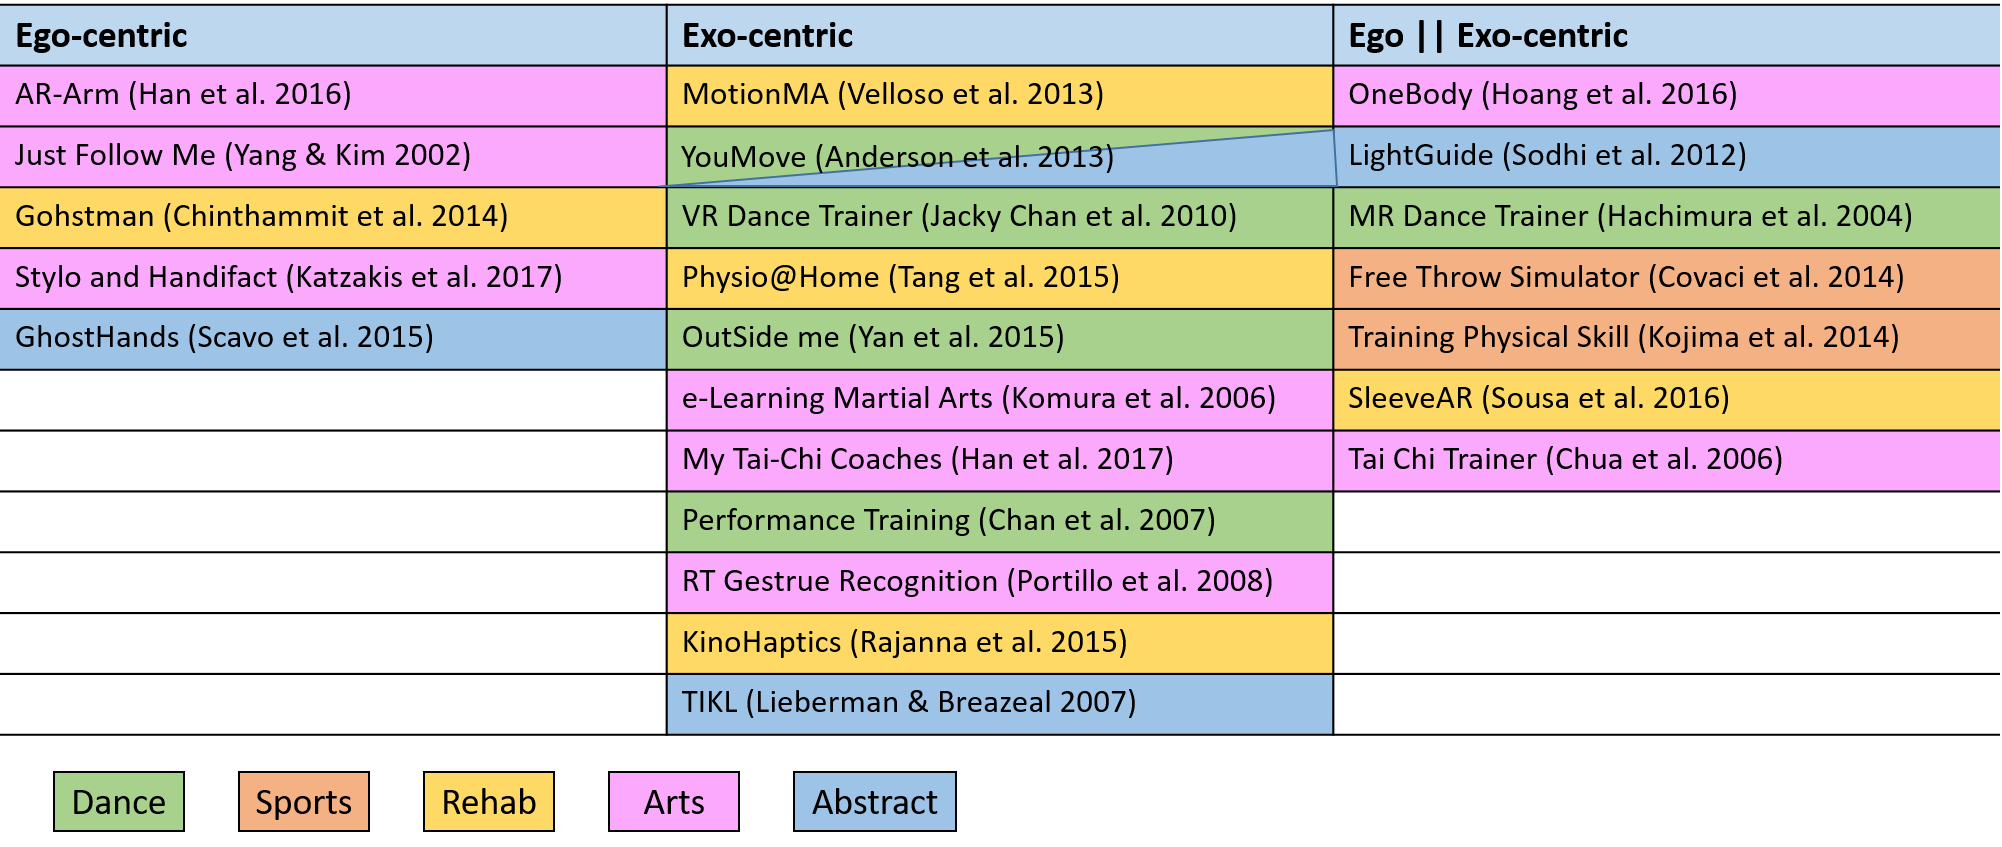
\includegraphics[width=\textwidth]{figures/rw_overview.png}
	\caption[Overview seminar evaluation]{Overview of related work divided by perspective and task}
	\label{tab:rw_overview}
\end{table}
\begin{table}[htb]
	\centering
	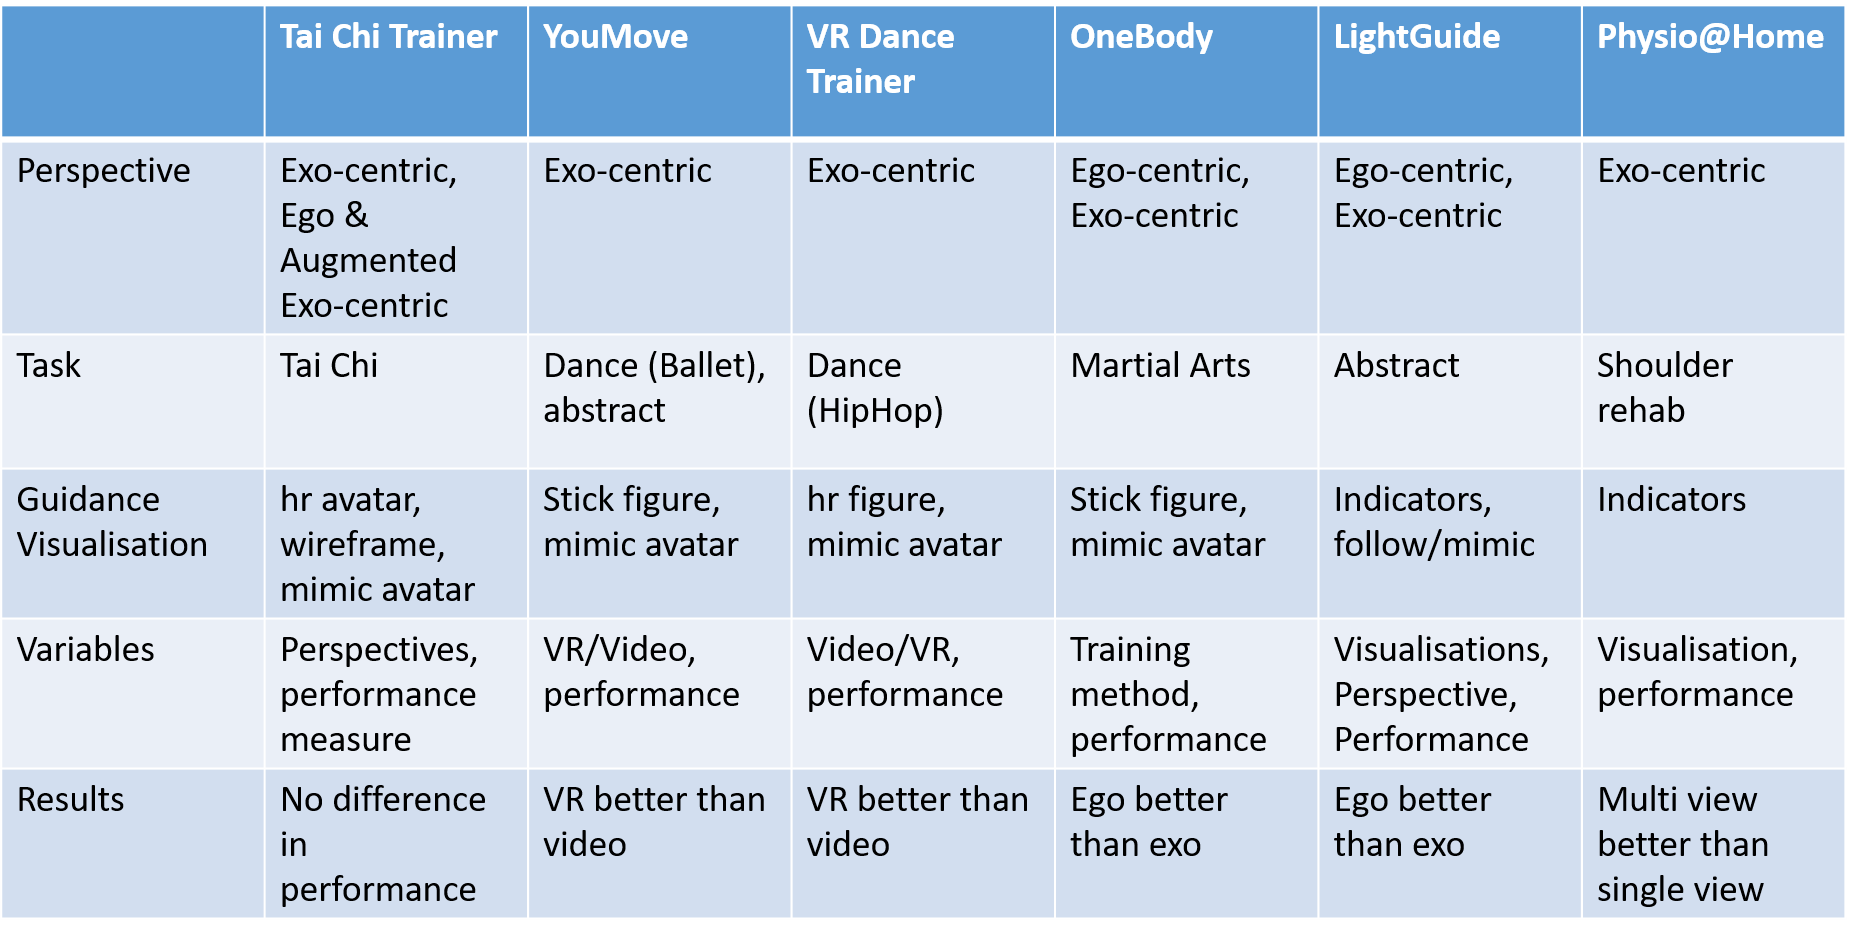
\includegraphics[width=\textwidth]{figures/detail_paper_overview.png}
	\caption[Detailed analysis of related work in seminar thesis.]{Detailed seminar thesis evaluation.}
	\label{tab:rw_overview_detail}
\end{table}
These works inform this work in various aspects. Chua et al. used the ego \& augmented exo-centric visual perspective, Hoang et al. and Sodhi et al. the ego-centric visual perspective. These visual perspectives proved to be suited for the evaluation of Motor Learning in VR and is adopted for the proposed study design, compare section~\ref{section:visual_perspectives}. Furthermore, Chan et al. and Chua et al. used high realistic avatars as guidance visualisation, which are used in the proposed study design, compare seminar thesis chapter 3.3. Additionally, recent research indicates that high realism avatars outperform abstract avatars~\cite{max,perspectivematters}. All authors used a performance measure to evaluate the performed movements of the participants of their studies. Primarily the distance-based measures informed the measures used in the proposed study design\\%compare figure ??? yxc
The above mentioned works do not use the relatively new technology of Vive Trackers in combination with Inverse Kinematics (IK, see project report chapter 2.1 and 2.2). Sra et al.~\cite{samesetup} used this technology in 2018 for their system Your Place and Mine to render human-shaped avatars.\\
The results of related work yielded no clear conclusion about the influence of the perspectives on motor learning. Chua et al. found no difference in the performance between the visual perspectives, Anderson et al. and Chan et al. found out that their exo-centric visual perspectives in Virtual Reality outperform traditional video guidance. Hoang et al. and Sodhi et al. conclude that the ego-centric perspective outperforms the exo-centric visual perspective. Nevertheless, an investigation of how the visual perspective influences motor learning was not investigated. Recently, in December 2020, Yu et al.~\cite{perspectivematters} conducted three independent studies to close this gap. In the first study, Yu et al. compared the ego-centric visual perspective and a 2D-mirror for single arm movements. In the second study, they compared the ego-centric and exo-centric visual perspective for Yoga. In the third study, they compared the ego-centric visual perspective with a 3D-mirror for arm movements. Yu et al. conclude their findings in a design guideline for systems training Motor Learning in Virtual Reality: use the ego-centric visual perspective if the type of motion allows, consider alternatives for other types of motions, ibidem. In all three studies, the ego-centric visual perspective outperformed the other perspectives if the movement was completely visible from the ego-centric visual perspective. This work, in contrast, focuses on full-body movements that include the handling of physical load. Furthermore, this work provides a third visual perspective, where the ego-centric and exo-centric visual perspective is combined.

\subsection{Research Contribution Statement}
\label{delimination_contribution}
\todo{new papers occured, read them, then write this statement. notes:}
what is done: 
comparing ego-centric with exo-centric video.
comparing ego-centric with exo-centric and the combination, but yielded to no result, because old paper and old pc
comparing with mirrors,
comparing isolated body parts
everyone made his live easy by just looking at stationary movements, mostly containing only some body parts.
new: nobody did fullbody movements with locomotion. ego-centric locomotion motion guidance is completely new. 
related work only investigated on stationary movements. but motor learning is not stationary. body parts is also not stationary.
real-world relation poor because of arts dance or abstract. my work is the first one haveing really a task that is reasonable!\\
Previous work investigated the differences between the perspectives, but:
To my knowledge, there is no investigation on full body movements that include locomotion. Furthermore, there are on investigations that include the handling of physical load.
Perivous works compared ego-centric Motor Learning with video learning\cite{YouMove,vrdancetrainer}, augemnted mirrors\cite{perspectivematters,onebody}.
The conduction of the proposed study will produce data that serves as a reasonable basis for designers of VR Motor Learning systems choosing a suitable perspectives. This is achieved by an Empirical Research Contribution. The empirical data is gathered by a comparative study between the ego-centric visual perspective, the exo-centric visual perspective and the combination. As novelty, the task includes handling of physical load which consists of the elemental tasks of manual material handling. This allows an evaluation of the elemental tasks per visual perspective and can give insights which perspective is suited for specific tasks.\\
Additionaly, an artifact contribution is provided by the ego-centric guidance of locomotion movements.


